\documentclass[a4paper]{article}

\usepackage{graphicx}
\usepackage{amsmath}
\usepackage{natbib}
\usepackage{amsmath}
\usepackage[english]{babel}
\usepackage{graphicx}
\usepackage{amssymb}
\usepackage{graphicx}
\usepackage{url}
\usepackage{listings}
\usepackage{paralist}
\usepackage{color}
\usepackage{epstopdf}

\date{}

\begin{document}

\section{Comparison Plots}

\begin{figure}[h!]
\centering
\begin{tabular}{cc}
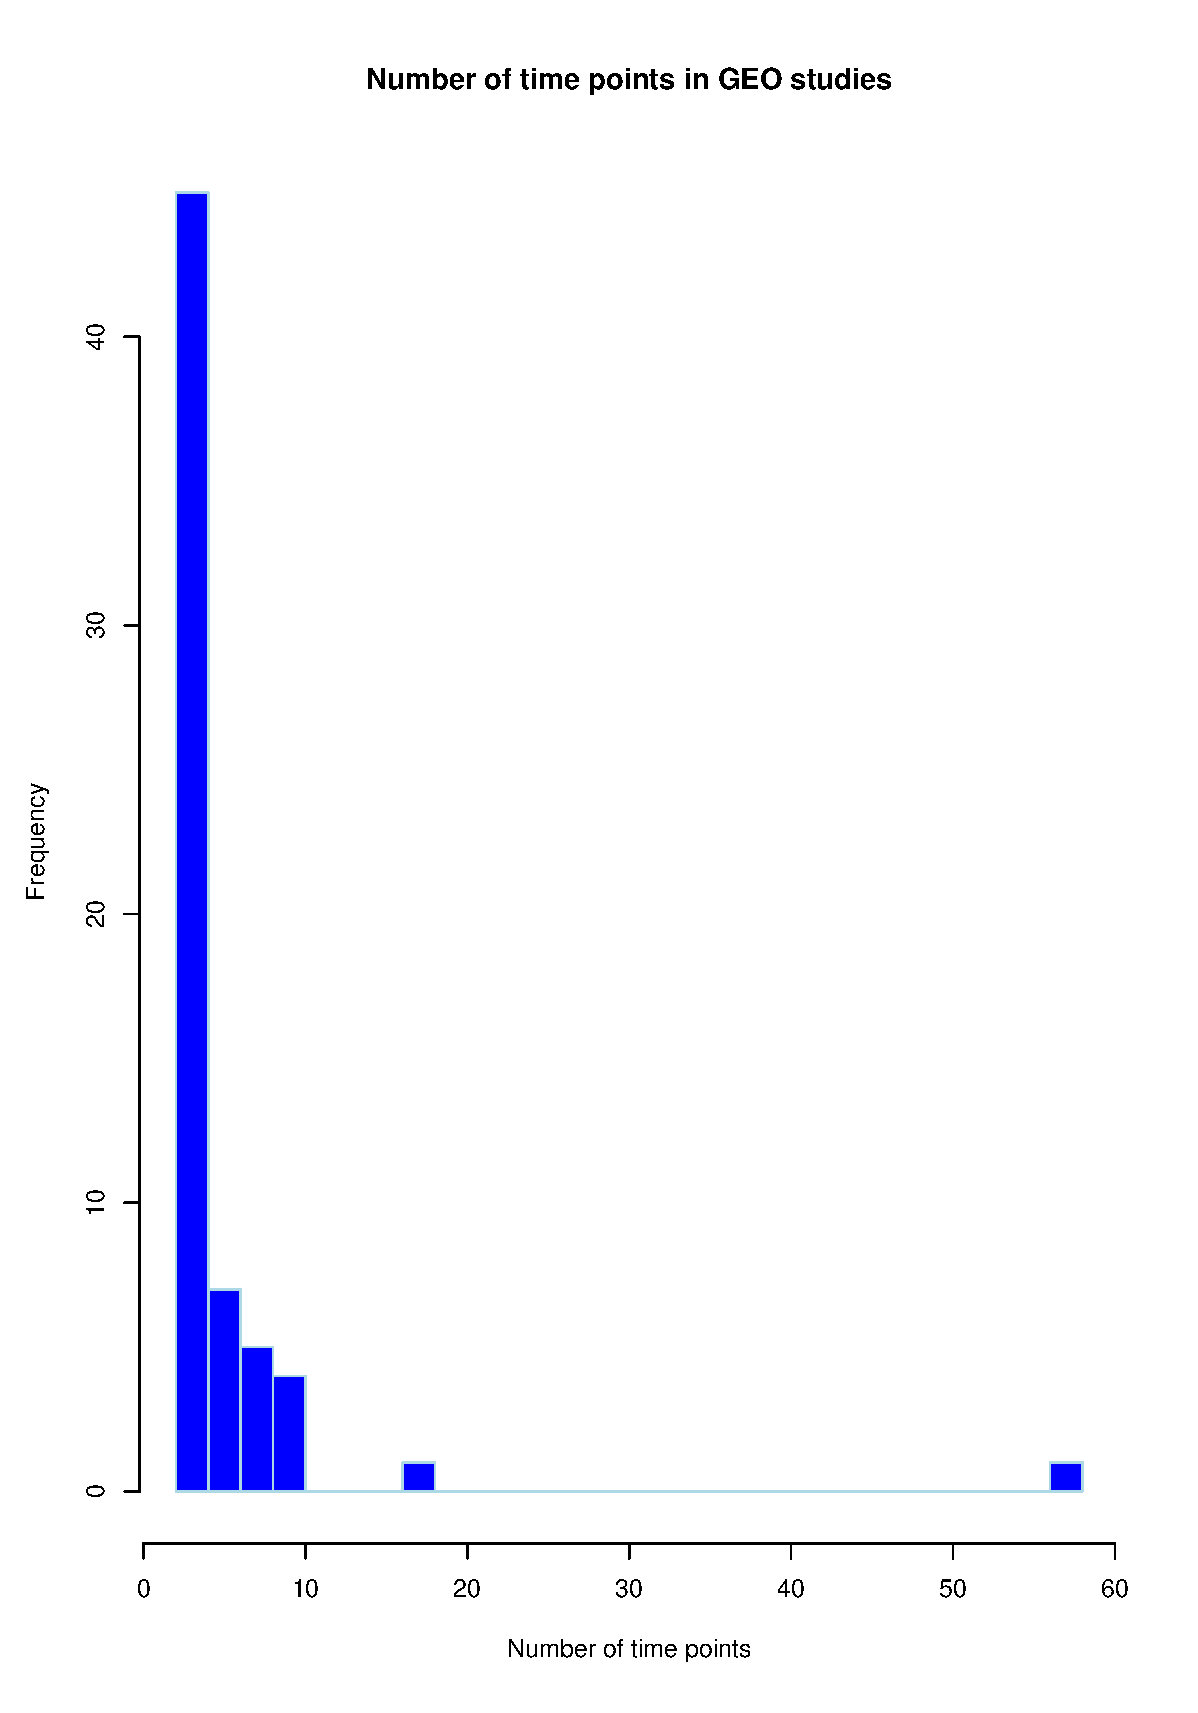
\includegraphics[scale=0.3]{GEOtime.eps}&
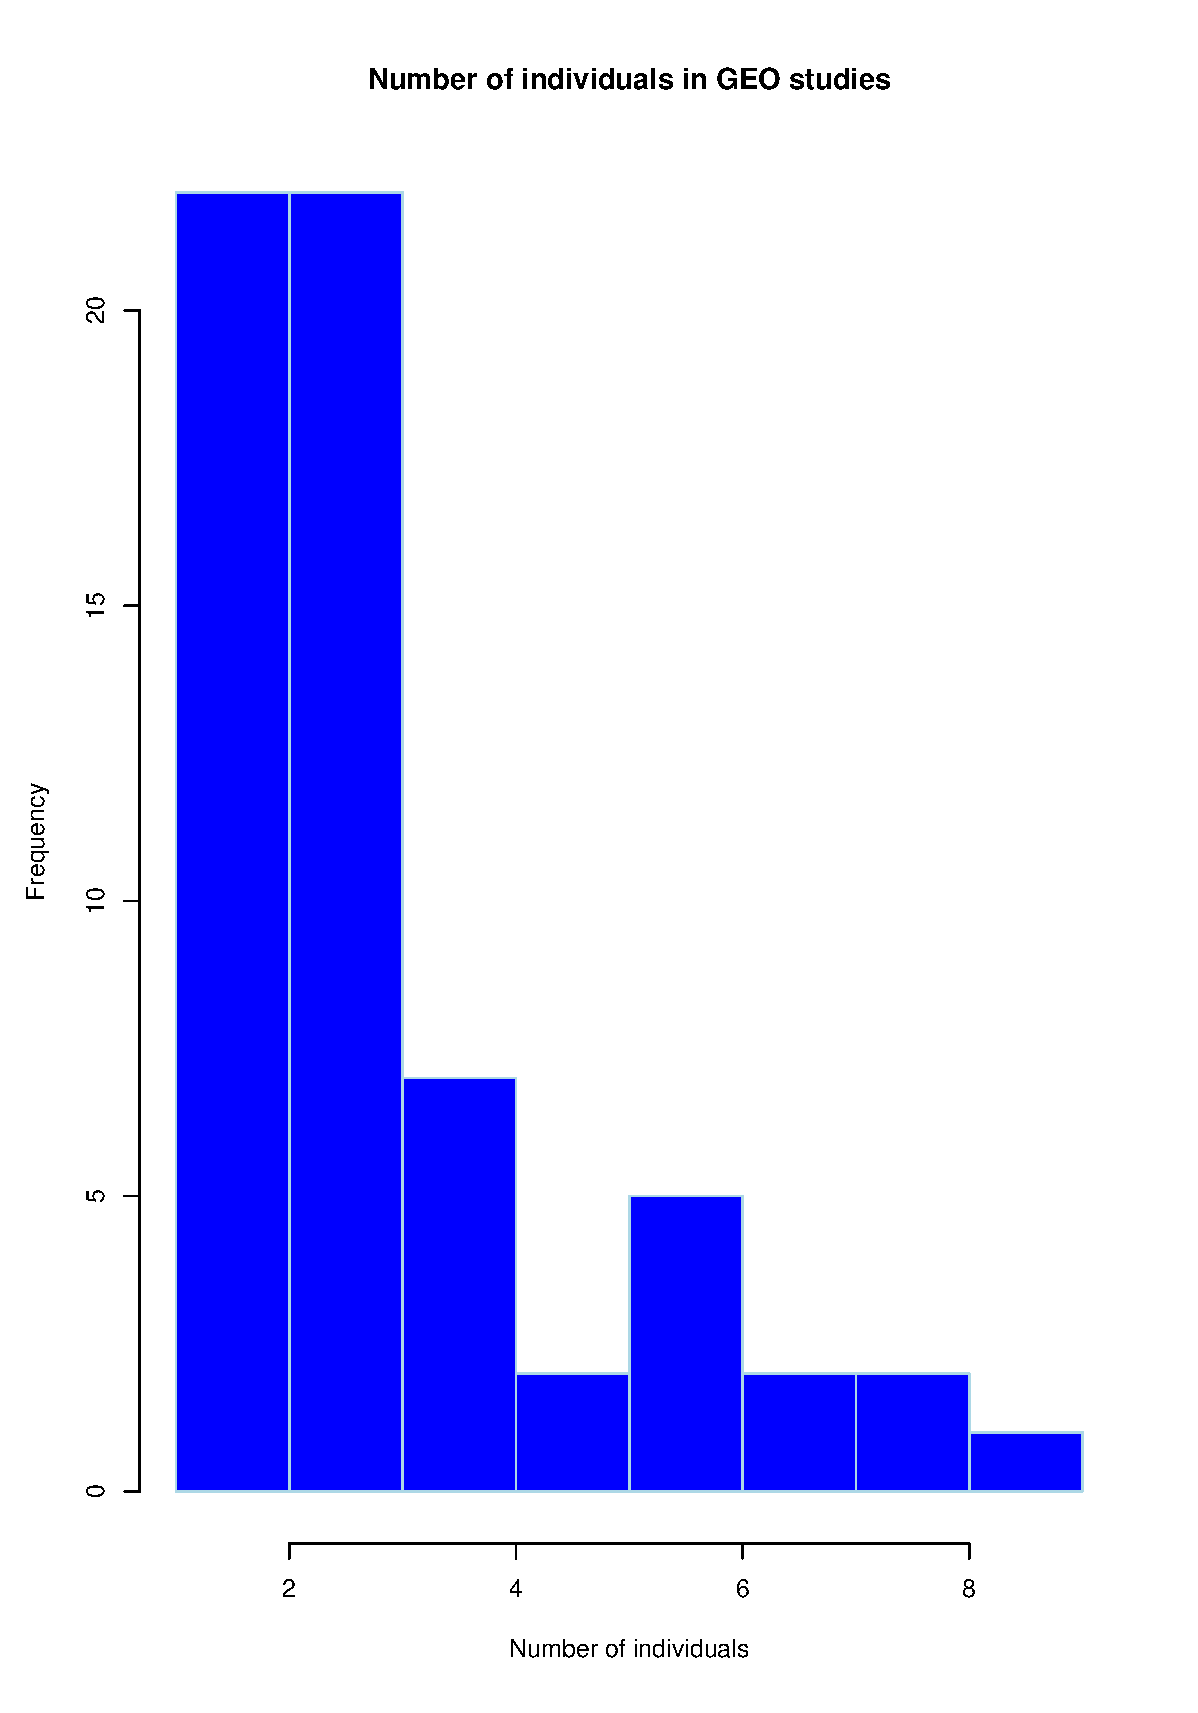
\includegraphics[scale=0.3]{GEOind.eps}\\
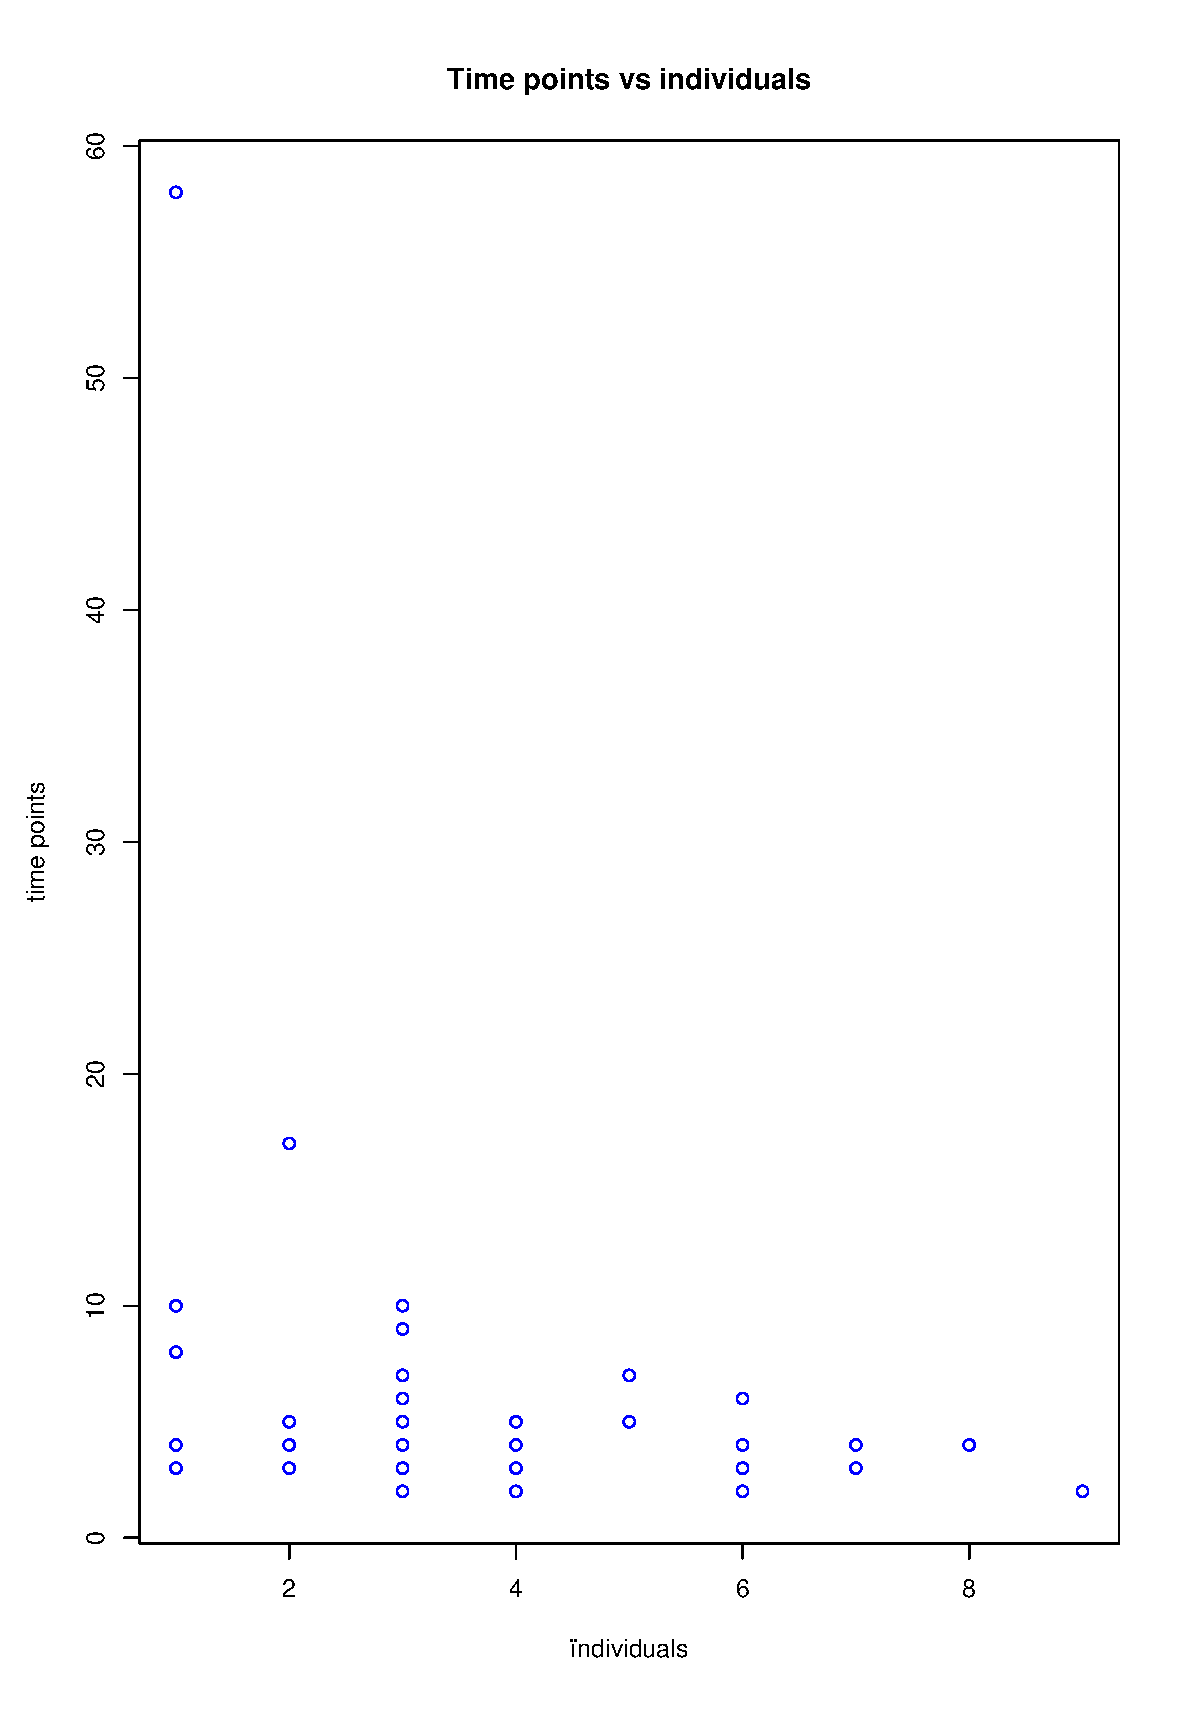
\includegraphics[scale=0.3]{GEOscat.eps}\\
\end{tabular}
\caption{Number of time-points and observations in microarray time-course gene expression studies from GEO database. Upper left panel represent histogram of number of time-points, while upper right panel illustrate histogram of observations in GEO studies. Lower panel show number of time points plotted against number of individuals.}
\label{fig:GEOhist}
\end{figure}


\begin{figure}[h!]
\centering
\begin{tabular}{cc}
\includegraphics[scale=0.5,angle=270]{LossA25T10N5.eps}\\
\includegraphics[scale=0.5,angle=270]{LossOmega25T10N5.eps}\\
\end{tabular}
\caption{Frobenius loss comparison between lasso and ridge estimators for precision and autoregressive coefficient matrix on simulated data set where p=25, T=10 and n=5.}
\label{fig:Loss25T10N5}
\end{figure}

\begin{figure}[h!]
\centering
\begin{tabular}{cc}
\includegraphics[scale=0.5,angle=270]{LossA50T10N5.eps}\\
\includegraphics[scale=0.5,angle=270]{LossOmega50T10N5.eps}\\
\end{tabular}
\caption{Frobenius loss comparison between lasso and ridge estimators for precision and autoregressive coefficient matrix on simulated data set where p=50, T=10 and n=5.}
\label{fig:Loss50T10N5}
\end{figure}
 
%%%%%%%%%%%%%%%%%%%%%%%%%%%%%%%%%%%%%%%%%%%%%%%%%%%%%%%%%%%%%%%%%%%%%%%%%%%%%%%%%%%%

\begin{figure}[h!]
\centering
\begin{tabular}{cc}
\includegraphics[scale=0.5,angle=270]{LossA25T20N5.eps}\\
\includegraphics[scale=0.5,angle=270]{LossOmega25T20N5.eps}\\
\end{tabular}
\caption{Frobenius loss comparison between lasso and ridge estimators for precision and autoregressive coefficient matrix on simulated data set where p=25, T=20 and n=5.}
\label{fig:Loss25T20N5}
\end{figure}

\begin{figure}[h!]
\centering
\begin{tabular}{cc}
\includegraphics[scale=0.5,angle=270]{LossA50T20N5.eps}\\
\includegraphics[scale=0.5,angle=270]{LossOmega50T20N5.eps}\\
\end{tabular}
\caption{Frobenius loss comparison between lasso and ridge estimators for precision and autoregressive coefficient matrix on simulated data set where p=50, T=20 and n=5.}
\label{fig:Loss50T20N5}
\end{figure}

%%%%%%%%%%%%%%%%%%%%%%%%%%%%%%%%%%%%%%%%%%%%%%%%%%%%%%%%%%%%%%%%%%%%%%%%%%%%%%%%%%

\begin{figure}[h!]
\centering
\begin{tabular}{cc}
\includegraphics[scale=0.5,angle=270]{LossA25T10N15.eps}\\
\includegraphics[scale=0.5,angle=270]{LossOmega25T10N15.eps}\\
\end{tabular}
\caption{Frobenius loss comparison between lasso and ridge estimators for precision and autoregressive coefficient matrix on simulated data set where p=25, T=10 and n=15.}
\label{fig:Loss25T20N5}
\end{figure}

\begin{figure}[h!]
\centering
\begin{tabular}{cc}
\includegraphics[scale=0.5,angle=270]{LossA50T10N15.eps}\\
\includegraphics[scale=0.5,angle=270]{LossOmega50T10N15.eps}\\
\end{tabular}
\caption{Frobenius loss comparison between lasso and ridge estimators for precision and autoregressive coefficient matrix on simulated data set where p=50, T=10 and n=15.}
\label{fig:Loss50T20N5}
\end{figure}

%%%%%%%%%%%%%%%%%%%%%%%%%%%%%%%%%%%%%%%%%%%%%%%%%%%%%%%%%%%%%%%%%%%%%%%%%%%%%%%%%%

\begin{figure}[h!]
\centering
\begin{tabular}{cc}
\includegraphics[scale=0.5,angle=270]{LossA25T20N15.eps}\\
\includegraphics[scale=0.5,angle=270]{LossOmega25T20N15.eps}\\
\end{tabular}
\caption{Frobenius loss comparison between lasso and ridge estimators for precision and autoregressive coefficient matrix on simulated data set where p=50, T=20 and n=15.}
\label{fig:Loss25T20N15}
\end{figure}

\begin{figure}[h!]
\centering
\begin{tabular}{cc}
\includegraphics[scale=0.5,angle=270]{LossA50T20N15.eps}\\
\includegraphics[scale=0.5,angle=270]{LossOmega50T20N15.eps}\\
\end{tabular}
\caption{Frobenius loss comparison between lasso and ridge estimators for precision and autoregressive coefficient matrix on simulated data set where p=50, T=20 and n=15.}
\label{fig:Loss50T20N15}
\end{figure}

%%%%%%%%%%%%%%%%%%%%%%%%%%%%%%%%%%%%%%%%%%%%%%%%%%%%%%%%%%%%%%%%%%%%%%%%%%%%%%%%%%

\begin{figure}[htb!]
\centering
\begin{tabular}{cc}
\includegraphics[scale=0.5,angle=270]{ROCfpr25T10N5a.eps}\\
\includegraphics[scale=0.5,angle=270]{ROCfpr25T10N5b.eps}\\
\end{tabular}
\caption{Box plot of specificity (false positive rate) of the methods on simulated data where p=25, T=10 and n=5. First panel displays comparison based on lasso selection(first type), while in second panel estimation and selection are performed separately(second type).}
\label{fig:fpr25T10N5}
\end{figure}

\begin{figure}[h!]
\centering
\begin{tabular}{cc}
\includegraphics[scale=0.5,angle=270]{ROCtpr25T10N5a.eps}\\
\includegraphics[scale=0.5,angle=270]{ROCtpr25T10N5b.eps}\\
\end{tabular}
\caption{Box plot of sensitivity (true positive rate) of the methods on simulated data where p=25, T=10 and n=5. First panel displays comparison based on lasso selection(first type), while in second panel estimation and selection are performed separately(second type).}
\label{fig:tpr25T10N5}
\end{figure}

\begin{figure}[h!]
\centering
\begin{tabular}{cc}
\includegraphics[scale=0.5,angle=270]{ROCfpr50T10N5a.eps}\\
\includegraphics[scale=0.5,angle=270]{ROCfpr50T10N5b.eps}\\
\end{tabular}
\caption{Box plot of specificity (false positive rate) of the methods on simulated data where p=50, T=10 and n=5.  First panel displays comparison based on lasso selection(first type), while in second panel estimation and selection are performed separately(second type).}
\label{fig:fpr50T10N5}
\end{figure}

\begin{figure}[h!]
\centering
\begin{tabular}{cc}
\includegraphics[scale=0.5,angle=270]{ROCtpr50T10N5a.eps}\\
\includegraphics[scale=0.5,angle=270]{ROCtpr50T10N5b.eps}\\
\end{tabular}
\caption{Box plot of sensitivity (true positive rate) of the methods on simulated data where p=50, T=10 and n=5. First panel displays comparison based on lasso selection(first type), while in second panel estimation and selection are performed separately(second type).}
\label{fig:tpr25T10N5}
\end{figure}
%%%%%%%%%%%%%%%%%%%%%%%%%%%%%%%%%%%%%%%%%%%%%%%%%%%%%%%%%%%%%%%%%%%%%%%%%%
%%%%%%%%%%%%%%%%%%%%%%%%%%%%%%%%%%%%%%%%%%%%%%%%%%%%%%%%%%%%%%%%%%%%%%%%%%
%%%%%%%%%%%%%%%%%%%%%%%%%%%%%%%%%%%%%%%%%%%%%%%%%%%%%%%%%%%%%%%%%%%%%%%%%%
\begin{figure}[h!]
\centering
\begin{tabular}{cc}
\includegraphics[scale=0.5,angle=270]{ROCfpr25T20N15a.eps}\\
\includegraphics[scale=0.5,angle=270]{ROCfpr25T20N15b.eps}\\
\end{tabular}
\caption{Box plot of specificity (false positive rate) of the methods on simulated data where p=25, T=20 and n=15. First panel displays comparison based on lasso selection(first type), while in second panel estimation and selection are performed separately(second type).}
\label{fig:fpr25T20N15}
\end{figure}

\begin{figure}[h!]
\centering
\begin{tabular}{cc}
\includegraphics[scale=0.5,angle=270]{ROCtpr25T20N15a.eps}\\
\includegraphics[scale=0.5,angle=270]{ROCtpr25T20N15b.eps}\\
\end{tabular}
\caption{Box plot of sensitivity (true positive rate) of the methods on simulated data where p=25, T=20 and n=15. First panel displays comparison based on lasso selection(first type), while in second panel estimation and selection are performed separately(second type).}
\label{fig:tpr25T20N15}
\end{figure}

\begin{figure}[h!]
\centering
\begin{tabular}{cc}
\includegraphics[scale=0.5,angle=270]{ROCfpr50T20N15a.eps}\\
\includegraphics[scale=0.5,angle=270]{ROCfpr50T20N15b.eps}\\
\end{tabular}
\caption{Box plot of specificity (false positive rate) of the methods on simulated data where p=50, T=20 and n=15. First panel displays comparison based on lasso selection(first type), while in second panel estimation and selection are performed separately(second type).}
\label{fig:fpr50T20N15}
\end{figure}

\begin{figure}[h!]
\centering
\begin{tabular}{cc}
\includegraphics[scale=0.5,angle=270]{ROCtpr50T20N15a.eps}\\
\includegraphics[scale=0.5,angle=270]{ROCtpr50T20N15b.eps}\\
\end{tabular}
\caption{Box plot of sensitivity (true positive rate) of the methods on simulated data where p=50, T=20 and n=15. First panel displays comparison based on lasso selection(first type), while in second panel estimation and selection are performed separately(second type).}
\label{fig:tpr50T20N15}
\end{figure}
 

\end{document}


@article{ernst2005clustering,
  title={Clustering short time series gene expression data},
  author={Ernst, Jason and Nau, Gerard J and Bar-Joseph, Ziv},
  journal={Bioinformatics},
  volume={21},
  number={suppl 1},
  pages={i159--i168},
  year={2005},
  publisher={Oxford Univ Press}
}

@article{Edgar2002,
  title={Gene Expression Omnibus: NCBI gene expression and hybridization array data repository},
  author={Edgar, Ron and Domrachev, Michael and Lash, Alex E},
  journal={Nucleic acids research},
  volume={30},
  number={1},
  pages={207--210},
  year={2002},
  publisher={Oxford Univ Press}
}

@article{Kanehisa2000,
  title={KEGG: kyoto encyclopedia of genes and genomes},
  author={Kanehisa, Minoru and Goto, Susumu},
  journal={Nucleic acids research},
  volume={28},
  number={1},
  pages={27--30},
  year={2000},
  publisher={Oxford Univ Press}
}

@article{Gentleman2004,
  title={Bioconductor: open software development for computational biology and bioinformatics},
  author={Gentleman, Robert C and Carey, Vincent J and Bates, Douglas M and Bolstad, Ben and Dettling, Marcel and Dudoit, Sandrine and Ellis, Byron and Gautier, Laurent and Ge, Yongchao and Gentry, Jeff and others},
  journal={Genome biology},
  volume={5},
 number={10},
  pages={R80},
  year={2004},
  publisher={BioMed Central Ltd}
}

  @Manual{Carey2015,
    title = {bronchialIL13: time course experiment involving il13},
    author = {Vince Carey},
    note = {R package version 1.3.1},
    url = {http://www.biostat.harvard.edu/~carey},
  }

@article{Steenbergen1996,
  title={Transition of human papillomavirus type 16 and 18 transfected human foreskin keratinocytes towards immortality: activation of telomerase and allele losses at 3p, 10p, 11q and/or 18q.},
  author={Steenbergen, RD and Walboomers, JM and Meijer, CJ and Van Der Raaij-Helmer, EM and Parker, Jacqueline N and Chow, Louise T and Broker, Thomas R and Snijders, PJ},
  journal={Oncogene},
  volume={13},
  number={6},
  pages={1249--1257},
  year={1996}
}

@article{Irizarry2003,
  title={Exploration, normalization, and summaries of high density oligonucleotide array probe level data},
  author={Irizarry, Rafael A and Hobbs, Bridget and Collin, Francois and Beazer-Barclay, Yasmin D and Antonellis, Kristen J and Scherf, Uwe and Speed, Terence P and others},
  journal={Biostatistics},
  volume={4},
  number={2},
  pages={249--264},
  year={2003}
}

@article{Huber2002,
  title={Variance stabilization applied to microarray data calibration and to the quantification of differential expression},
  author={Huber, Wolfgang and Von Heydebreck, Anja and S{\"u}ltmann, Holger and Poustka, Annemarie and Vingron, Martin},
  journal={Bioinformatics},
  volume={18},
  number={suppl 1},
  pages={S96--S104},
  year={2002},
  publisher={Oxford Univ Press}
}

@article{Joshi2005,
  title={Reactome: a knowledgebase of biological pathways},
  author={Joshi-Tope, G and Gillespie, Marc and Vastrik, Imre and D'Eustachio, Peter and Schmidt, Esther and de Bono, Bernard and Jassal, Bijay and Gopinath, GR and Wu, GR and Matthews, Lisa and others},
  journal={Nucleic acids research},
  volume={33},
  number={suppl 1},
  pages={D428--D432},
  year={2005},
  publisher={Oxford Univ Press}
}

@article{Miok2014,
  title={tigaR: integrative significance analysis of temporal differential gene expression induced by genomic abnormalities},
  author={Miok, Viktorian and Wilting, Saskia M and van de Wiel, Mark A and Jaspers, Annelieke and van Noort, Paula I and Brakenhoff, Ruud H and Snijders, Peter JF and Steenbergen, Renske DM and van Wieringen, Wessel N},
  journal={BMC bioinformatics},
  volume={15},
  number={1},
  pages={327},
  year={2014},
  publisher={BioMed Central Ltd}
}

@Manual{Ligtenberg2015,
    title = {reactome.db: A set of annotation maps for reactome},
    author = {Willem Ligtenberg},
    note = {R package version 1.48.0},
  }
